\subsection{Statistical analysis of experiment 2}
In this section the analysis of the results from experiment 2 will be conducted. Firstly the normal distribution for experiment 2 will be analyzed using the Shapiro-Wilk test. 

The expectations is that the distribution wil not be normally distributed, this is because experiment 1 was not always normally distributed, we would not expected this experiment to differ much in that aspects. 

\begin{table}[]
    \begin{tabular}{||c|c|c|c|c|c||}    \hline
    &\textbf{TestCaseIdle}&\textbf{BinaryTrees}&\textbf{FannkuchRedux}&\textbf{Nbody}&\textbf{Fasta}\\ [0.5ex] \hline
    \hline \textbf{IntelPowerGadget}&0.0&0.9103&0.1293&0.0002&0.8291\\
    \textbf{HardwareMonitor}&0.0213&0.1345&0.0492&0.3209&0.0\\
    \textbf{Clamp Win}&0.0034&0.0023&0.012&0.8143&0.5335\\
    \textbf{RAPL}&0.1899&0.5744&0.0015&0.9437&0.0518\\
    \textbf{Clamp Lin}&0.4601&0.0004&0.0&0.1006&0.0002\\ \hline \end{tabular}
    \caption{P values for the normal distribution for the Workstation in Ex2}
    \label{tab:NormDist2}
\end{table} 

As can be seen in \cref{tab:NormDist2}, the data is not normally distributed the data from experiment 2 is generally further away from being normally distributed than the experiment 1. This is not that surprising given that experiment 2 contain less actual runs as these were not needed as found in \cref{subsec:CockUse}. 

For the MannWhitney U test we would again expect very similar results to the results from experiment one, where the null hypotheses can be rejected in most of the cases.
The results from the MannWhitney U test can be seen here in \cref{tab:HeatFannkuchRedux2}.
\begin{figure}
    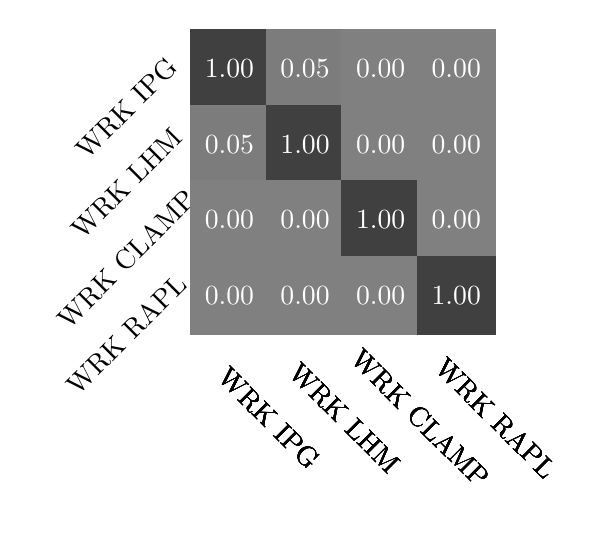
\begin{tikzpicture}[scale=0.6]
      \foreach \y [count=\n] in {{1.00, 0.05, 0.00, 0.00},{0.05, 1.00, 0.00, 0.00},{0.00, 0.00, 1.00, 0.00},{0.00, 0.00, 0.00, 1.00},} {
      % column labels
      \foreach \a [count=\n] in {WRK IPG,WRK LHM,WRK CLAMP,WRK RAPL} {
        \node[minimum size=10mm, xshift=0.5cm, rotate=-45] at (\n*1.6, -9.0) {\a};
      }
      % heatmap tiles
      \foreach \x [count=\m] in \y {
        \pgfmathsetmacro{\xa }{(\x + 1) / 2 * 100}
        \node[fill=darkgray!\xa!lightgray, minimum size=10mm, text=white, font={\normalsize}] at (\m*1.6,-\n*1.6) {\x};
      }
    }
      % row labels
      \foreach \a [count=\i] in {WRK IPG,WRK LHM,WRK CLAMP,WRK RAPL} {
        \node[minimum size=10mm, xshift=-0.35cm, yshift=-0.5cm, rotate=45] at (0,-\i*1.6) {\a};
      }
    \end{tikzpicture}
    \label{tab:HeatFannkuchRedux2}
\end{figure}
The shown table in \cref{tab:HeatFannkuchRedux2}, is again from the FannkuchRedux Test Case as in \cref{subsec:Stat1}. Again we see a similar tendency in that for most cases we can reject $H_0$, but for experiment 2 there are a few more cases where we cannot reject $H_0$. Once possible reason why that might be the case is that there are fewer samples in experiment 2 so outlier have a larger effect on the Ex1Statistics.

Finally for the Correlations between the measuring instruments, the expectations for the correlations in Experiment 2 is that they are either are a bit more correlated since the uncertainty's of the C-Stats have been removed, or that i will remain nearly exactly the same. The calculated Correlations for experiments 2 can be seen in \cref{tab:correlationWork2}.
\begin{figure}
    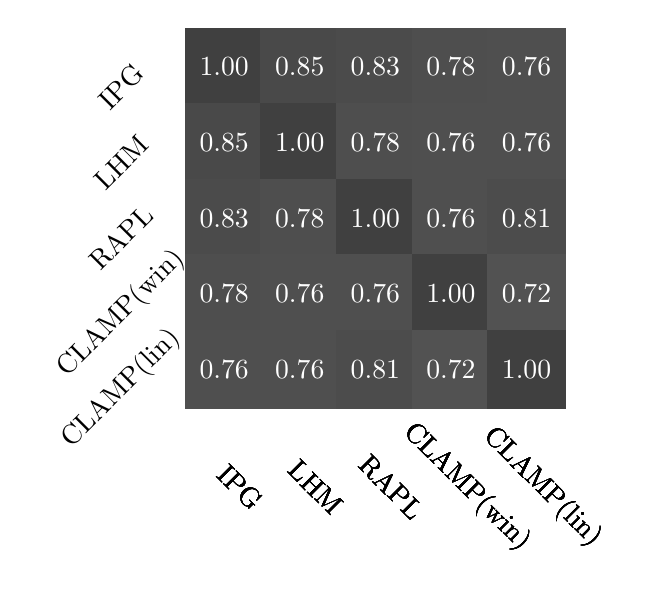
\begin{tikzpicture}[scale=0.6]
      \foreach \y [count=\n] in {{1.00, 0.85, 0.83, 0.78, 0.76},{0.85, 1.00, 0.78, 0.76, 0.76},{0.83, 0.78, 1.00, 0.76, 0.81},{0.78, 0.76, 0.76, 1.00, 0.72},{0.76, 0.76, 0.81, 0.72, 1.00},} {
      % column labels
      \foreach \a [count=\n] in {IPG,LHM,RAPL,CLAMP(win),CLAMP(lin)} {
        \node[minimum size=10mm, xshift=0.2cm, rotate=-45] at (\n*1.6, -10.5) {\a};
      }
      % heatmap tiles
      \foreach \x [count=\m] in \y {
        \pgfmathsetmacro{\xa }{(\x + 1) / 2 * 100}
        \node[fill=darkgray!\xa!lightgray, minimum size=10mm, text=white, font={\normalsize}] at (\m*1.6,-\n*1.6) {\x};
      }
    }
      % row labels
      \foreach \a [count=\i] in {IPG,LHM,RAPL,CLAMP(win),CLAMP(lin)} {
        \node[minimum size=10mm, xshift=-0.35cm, yshift=-0.25cm, rotate=45] at (0,-\i*1.6) {\a};
      }
    \end{tikzpicture}
    \label{tab:correlationWork2}
\end{figure}
At an first these results look very similar to the once from experiment 1, but to verify these number more in depth we can compare the averages of the correlations as before.

The average correlation from experiments on the workstation are:
$$AvgCoefEx1 = (0.81+0.80+0.77+0.71+0.80+0.78+0.71+0.77+0.72+0.70)/10 = 0.757$$
$$AvgCoefEx2 = (0.85+0.83+0.78+0.76+0.78+0.76+0.76+0.76+0.81+0.72)/10 = 0.781$$

This slight increase in overall correlation matches up with our expectations as the added consistency in the experiments should help reduce inconsistencies. Generally the correlations are higher in experiment 2, but the correlation does fall in certain cases, these cases will be looked at a bit here.

The first case is the $RAPL|CLAMP(win)$ which used to in experiment one to have a coefficients of $0.77$, but in Experiment 2 as $0.76$, while this is only a marginal decrease it could be caused by the fact that one measures linux and the other windows. Another one is $LHM|RAPL$ which went from $0.80$ to $0.78$ these measurements are again done on separate OSs. 

So the divide between linux and windows seems to have gotten larger.   









